\documentclass[twocolumn,10pt,final]{asme2ej}



%% End of ecrc-specific commands
%%%%%%%%%%%%%%%%%%%%%%%%%%%%%%%%%%%%%%%%%%%%%%%%%%%%%%%%%%%%%%%%%%%%%%%%%%

%% The amssymb package provides various useful mathematical symbols
\usepackage{amssymb}
%% The amsthm package provides extended theorem environments
%\usepackage{amsthm}
\usepackage{amsmath}
\usepackage{gensymb}

\usepackage[hidelinks]{hyperref}

% if you have landscape tables
\usepackage[figuresright]{rotating}

\begin{document}

\begin{center}

\textbf{\large{Pulse Height Spectra Analysis of a Neutron Energy Tuning Assembly}}

\noindent
\begin{tabular}{l}
\rule{3.2in}{0.02in}
\end{tabular}

{Jason R. Stickney$^1$, James E. Bevins$^1$, Edward Cazalas$^1$, John W. McClory$^1$}
\vspace{0.1in}

{[1] Department of Engineering Physics\\
	Air Force Institute of Technology,	WPAFB, OH 45433\\}

\end{center}

%%%%%%%%%%%%%%%%%%%%%%%%%%%%
%	Abstract
%%%%%%%%%%%%%%%%%%%%%%%%%%%%
\vspace{-0.5 cm}
\section*{Abstract}
\textbf{
Neutron spectrum shaping is a novel method that can be used to generate synthetic debris for nuclear forensics applications.  
An energy tuning assembly (ETA) was previously designed and built for the purpose of irradiating samples with a combination of a thermonuclear and a prompt fission neutron spectrum for production of synthetic debris for technical nuclear forensics at the National Ignition Facility. 
Initial bench-marking of the ETA performance was performed at the Lawrence Berkeley National Laboratory 88-Inch Cyclotron using 33 MeV deuteron breakup on tantalum as the neutron source.  
This research analyzes detector responses collected from three EJ-309 detectors used to characterize the ETA generated neutron field.   
Full waveform data from the source and ETA modified field were taken.  
A signal processing chain was developed to reduce the waveform data into a neutron only pulse height spectrum to unfold the measured neutron energy spectrum.}


%%%%%%%%%%%%%%%%%%%%%%%%%%%%
%	Introduction
%%%%%%%%%%%%%%%%%%%%%%%%%%%%
\vspace{-0.4 cm}
\section{Introduction} \label{intro}

Previous research developed a novel approach to designing neutron energy tuning assemblies (ETAs) to create customizable neutron spectra using existing facilities to address capability gaps that exist for many applications \cite{Bevins2017}.  
One such application is the creation of synthetic debris for post-detonation technical nuclear forensics (TNF) missions, specifically the creation of realistic synthetic fission and activation products that provide the characteristic ``fingerprint" used to aid in the attribution of weapon's origin  \cite{111thCongress2010, JNFWG2013}.
An ETA was designed to modify the National Ignition Facility (NIF) neutron source to have the spectral characteristics required to produce synthetic debris.
This research aims to benchmark the performance of the ETA to facilitate future experiments on NIF.  


%%%%%%%%%%%%%%%%%%%%%%%%%%%%
%	EXP Setup
%%%%%%%%%%%%%%%%%%%%%%%%%%%%
\vspace{-0.4 cm}
\section{Experimental Set-up} \label{sec:exp-setup}
The 88-Inch Cyclotron at LBNL is a variable energy, high-current, multi-particle cyclotron capable of accelerating deuterons up to a maximum energy of 65 MeV with maximum currents on the order of 10~particle-$\mu$ A. 
For the ETA experiments, a beam was designed to have a neutron spectrum that is peaked near 14 MeV -- NIF-relevant energies thereby probing the same interaction mechanisms -- and with a limited high energy component ($\sim$~0.5\% of the total fluence is above 20 MeV).
This was accomplished using a $^2$H$^+$ beam accelerated to 33~MeV and directed at a tantalum breakup target.
The deuteron beam was run at a current of $\sim$ 100~nA during the source beam  irradiation and $\sim$ 2~$\mu$A during the ETA irradiation. 
The beam was directed along the Cave~0 beam line and optically aligned using a phosphor located in the Cave~01 beam box, as shown in \autoref{explayout}. 
A Faraday cup located inside the cyclotron vault was equipped with a 4~mm thick tantalum breakup target along the Cave~0 beam line \cite{Bleuel2007}. 
The tantalum target is backed by a 14.5 mm thick copper cooling assembly with a 38~mm radius cutout centered on the tantalum target. 
The resulting neutrons and photons entering the experimental area were collimated by $\sim$ 3~m of concrete and $\sim$ 1.5~m of sand bags encasing the beam pipe, producing a high contrast, open-air neutron beam in the Cave~02 experimental area.

\vspace{-0.4 cm}
\begin{figure} [htp!]
\centering
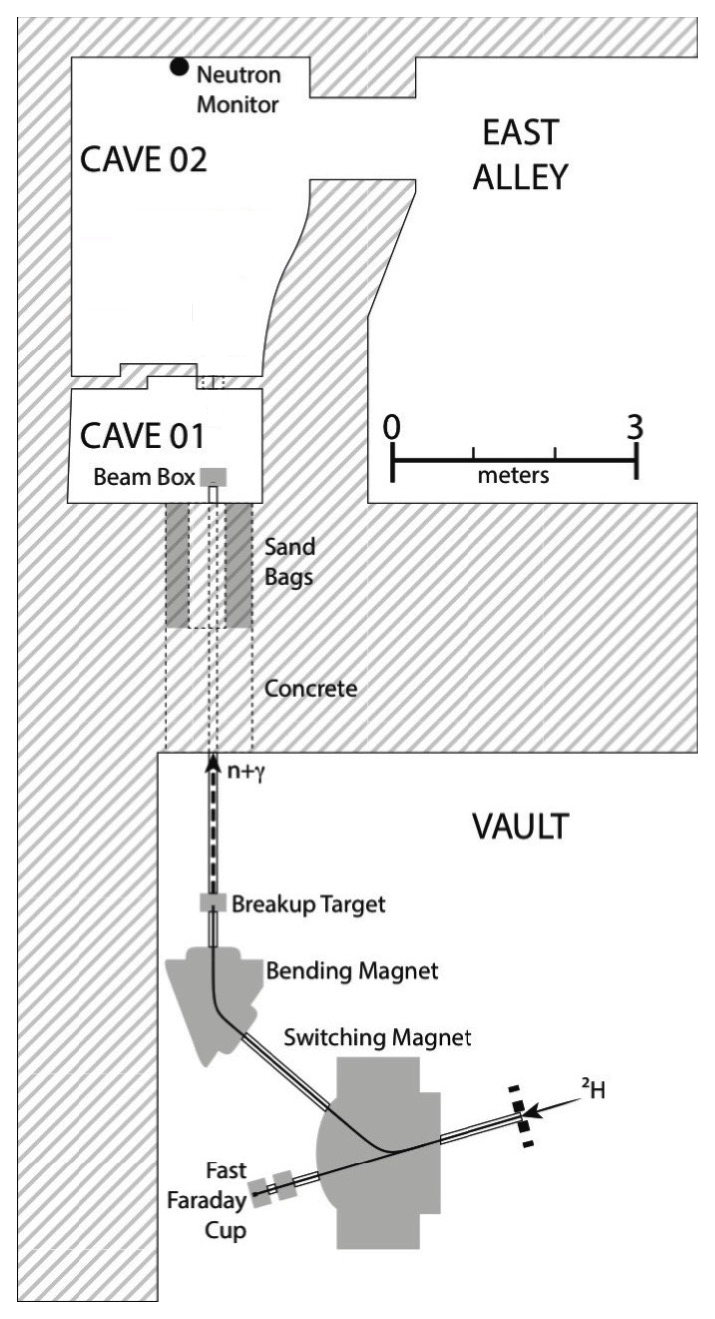
\includegraphics[width=0.28\textwidth]{../figs/vault_scaled.eps}
\caption{Schematic representation of the 88-Inch Cyclotron vault and beam line to Cave~0. The Cave~0 experimental end station is comprised of two enclosures, Cave~01 and Cave~02, separated by a lead-lined door outfitted with a beam port.}
\label{explayout}
\vspace{-0.4 cm}
\end{figure}

A cross-sectional view of the ETA designed for TNF applications is shown in \autoref{ETA}.
The outer diameter is 280~mm, the overall length is 240.2~mm, and the central sample cavity is 8.93~mm high with a diameter of 53.1~mm.

%\vspace{-0.4 cm}
\begin{figure} [htp!]
 \centering
 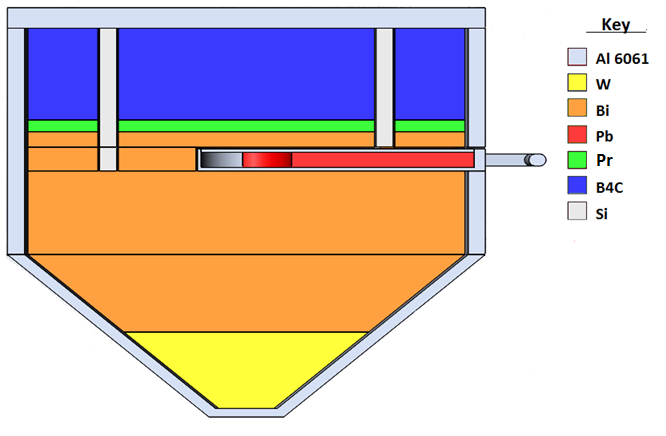
\includegraphics[trim = 0cm 0cm 0cm 0cm, clip, width=0.41\textwidth]{../Figs/ETA.png}
   \caption{Final ETA design \cite{Bevins2017}.}
     \label{ETA}
\vspace{-0.4 cm}
\end{figure}


The ETA was fielded in Cave~02 and plaed at beam line center (BLC) and 693.6~cm from the front face of the breakup target ($\sim$46.4~cm from the Cave~02 side of the Cave~01/Cave~02 wall shown in \autoref{explayout}).
Three EJ-309 detectors were arranged around the ETA to measure the ETA modified neutron field.
All were aligned in height with BLC and placed at angles of 0$\degree$, 45$\degree$, and 90$\degree$ with respect to the incident beam.  


%%%%%%%%%%%%%%%%%%%%%%%%%%%%
%	Results
%%%%%%%%%%%%%%%%%%%%%%%%%%%%
\vspace{-0.4 cm}
\section{Results} \label{sec:results}
The ratio of neutrons to gammas is $\sim$1:1 for 33~MeV deuteron breakup on a Ta target thereby requiring the use of pulse shape discrimination (PSD) to separate out the detector neutron response.
To improve discrimination at low pulse height (PH) events near the software threshold, optimization of the PSD parameters for the tail-to-total, tail-to-peak, and 90-10 methods were performed for each detector channel and data set.  
An example optimized PSD plot obtained for the detector at 0$\degree$ with the ETA using the tail-to-peak method is shown in \autoref{PSD}. 

\vspace{-0.5 cm}
\begin{figure} [htp!]
 \centering
 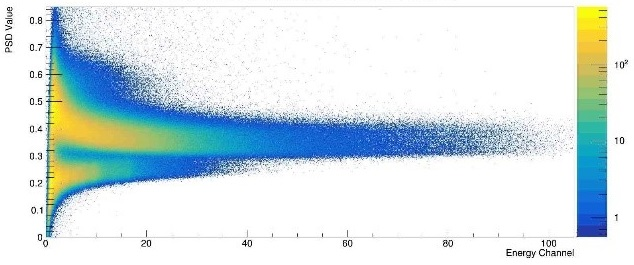
\includegraphics[trim = 0cm 0cm 0cm 0cm, clip, width=0.5\textwidth]{../Figs/psd.jpg}
   \caption{Uncalibrated PSD Histogram for the detector at 0$\degree$ with the ETA in place. The peak window used was 20 ns, and the tail window was 56 ns with a start off-set of 28 ns.}
  \label{PSD}
\vspace{-0.4 cm}
\end{figure}

A slice of \autoref{PSD} at the PH cutoff (channel 1305) is shown in \autoref{PSD-proj}.
Fitted cuts are developed to separate the neutron and gamma contributions resulting in the PH spectrum (PHS) shown in \autoref{PHS} for the three detectors with the ETA in place.

\vspace{-0.5 cm}
\begin{figure} [htp!]
 \centering
 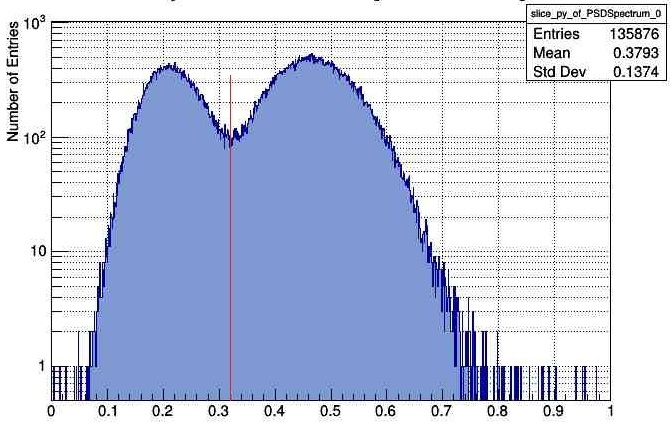
\includegraphics[trim = 0cm 0cm 0cm 0cm, clip, width=0.41\textwidth]{../Figs/psd-proj.jpg}
   \caption{PSD histogram near PH software threshold (channel 1305).}
  \label{PSD-proj}
\vspace{-0.5 cm}
\end{figure}

\vspace{-0.5 cm}
\begin{figure} [htp!]
 \centering
 \includegraphics[trim = 0cm 0cm 0cm 0cm, clip, width=0.41\textwidth]{../Figs/uncal-phs-allCh.png}
   \caption{Neutron PHS for the ETA measurements and all detectors.}
  \label{PHS}
\vspace{-0.4 cm}
\end{figure}

%%%%%%%%%%%%%%%%%%%%%%%%%%%%
%	Future Work
%%%%%%%%%%%%%%%%%%%%%%%%%%%%
\vspace{-0.4 cm}
\section{Future Work} \label{sec:future-work}

Analysis of this data is ongoing.
It is anticipated that the calibrated PH unfolding will be complete and neutron energy spectra for the source beam and ETA modification at all detector positions will be presented at the conference.
Additionally, comparisons with existing full-scale simulations to assess the ability to model ETA performance will be shown. 


%%%%%%%%%%%%%%%%%%%%%%%%%%%%
%	Acknowledgements
%%%%%%%%%%%%%%%%%%%%%%%%%%%%
\vspace{-0.4 cm}
\section*{Acknowledgments}
This material is based upon work supported in part by the Department of Energy National Nuclear Security Administration through the Nuclear Science and Security Consortium under Award Number DE-NA0003180, and performed under the auspices of the U.S. Department of Energy by Lawrence National Security, LLC, Lawrence Livermore National Laboratory under Contract DE-AC52-07NA27344. 
This work is also supported by the Lawrence Berkeley National Laboratory under Contract No. DE-AC02-05CH11231 for the US Nuclear Data Program and the National Science Foundation Graduate Research Fellowship under Grant No. NSF 11-582.
Additionally, the authors would like to thank the Bay Area Neutron Group at the University of California, Berkeley for their contributions to the analysis software.

%%%%%%%%%%%%%%%%%%%%%%%%%%%%
%	Disclaimer
%%%%%%%%%%%%%%%%%%%%%%%%%%%%
\vspace{-0.3 cm}
\section*{Disclaimer}
The views expressed in this thesis are those of the author and do not reflect the official policy or position of the United States Air Force, Department of Defense, or the United States Government.  This material is declared a work of the U.S. Government and is not subject to copyright protection in the United States.

%% References
%%
%% Following citation commands can be used in the body text:
%% Usage of \cite is as follows:
%%   \cite{key}         ==>>  [#]
%%   \cite[chap. 2]{key} ==>> [#, chap. 2]
%%

%% References with BibTeX database:

\vspace{-0.3 cm}
\bibliographystyle{elsarticle-num}
\bibliography{library}

%% Authors are advised to use a BibTeX database file for their reference list.
%% The provided style file elsarticle-num.bst formats references in the required Procedia style

%% For references without a BibTeX database:

% \begin{thebibliography}{00}

%% \bibitem must have the following form:
%%   \bibitem{key}...
%%

% \bibitem{}

% \end{thebibliography}

\end{document}

%%
%% End of file `ecrc-template.tex'. 